\section{Experiments}
\label{sec:exp}

% ─────────────────────────────────────────────────────────────────────────────
\subsection{Experimental Setup}
\label{sec:exp:setup}

\paragraph{Model and hardware}
All experiments use Klein~9B (MM-DiT architecture, 8 double-stream + 24
single-stream blocks, 32 layers total) via the DiffSynth backend, run in
bf16 mixed precision on a single H200 GPU.
Outputs are generated at $512 \times 512$ resolution with 25 denoising steps,
guidance scale~3.5, and fixed seed~43.
No model parameters are modified.

\paragraph{Benchmark construction}
We assemble a benchmark of 40 style references
(\texttt{sty/00}--\texttt{sty/39}) curated to span the breadth of visual styles a
training-free method must handle: traditional media (oil impasto, watercolor, ink
line art, bronze relief, ukiyo-e), graphic and illustrative styles (flat-color
posters, screenprint, art-deco, constructivist propaganda, comic), digital and
pixel art, and photographic textures. References were chosen for mutual visual
distinctness so that style fidelity is not inflated by near-duplicate references.
We exclude \texttt{sty04} from all T2I evaluation because its near-uniform pixel
statistics make the CSD embedding degenerate, leaving 39 styles.
% 十修: 删除过期表述"I2I additionally excludes sty14 and content cnt19 as
% pathological edge cases"——与事实矛盾: I2I 消融子集的 8 风格
% (00/10/14/20/27/28/33/38) 本身即含 sty14 (见下方 Evaluation splits 段)，
% 完整 741-pair I2I benchmark (39 styles x 19 contents, 见本文件 "full
% 741-pair I2I benchmark" 处) 同样不排除 sty14，且 cnt19 不存在于 19 个
% content 编号 (00--18) 范围内。该句为旧协议残留，予以删除。
The
six T2I content prompts (Table~\ref{tab:prompts}) are fixed in advance to span
object, animal, still-life, landscape, and architectural categories, decoupling
measured style fidelity from any single content type. The full style bank is
shown in the supplement (Fig.~\ref{fig:benchmark_atlas}).

\paragraph{Evaluation splits}
\emph{T2I} pairs every retained style with all six prompts
($39 \times 6 = 234$ pairs). \emph{Ablations and sweeps} use a 40-sample
subset---8 styles (\texttt{sty} 00/10/14/20/27/28/33/38) $\times$ 5 prompts
(\texttt{kp0}--\texttt{kp4})---chosen to span the style categories above while
permitting rapid iteration; the multi-seed robustness study reuses this subset.
\emph{I2I} uses a 40-pair subset: the same 8 styles $\times$ 5 content images
(\texttt{cnt} 00/04/08/12/17).

\begin{table}[h]
  \centering
  \caption{T2I benchmark content prompts.}
  \label{tab:prompts}
  \small
  \begin{tabular}{ll}
    \toprule
    ID & Prompt \\
    \midrule
    p0 & A cat sitting on a wooden table \\
    p1 & A sports car on a mountain road \\
    p2 & A field of sunflowers at sunset \\
    p3 & A dog running in a park \\
    p4 & A snowy mountain peak at dawn \\
    p5 & Portrait of a young woman \\
    \bottomrule
  \end{tabular}
\end{table}

\paragraph{Metrics}
We report three metrics, uniformly applied across all experiments.
\textbf{CSD}~($\uparrow$), the Contrastive Style Descriptor
similarity~\cite{somepalli2024measuring} between output and style reference,
serves as the primary style-fidelity metric.
\textbf{CLIP-T}~($\uparrow$), the CLIP ViT-B/32~\cite{radford2021learning}
image-text cosine similarity between output and content prompt,
measures content preservation.
\textbf{Forward passes / step}~($\downarrow$) counts the number of model forward
passes per denoising step, a hardware-agnostic efficiency metric; wall-clock
timing (each Adam iteration—one forward plus one backward pass per denoising
step—adds $\approx$2.1~s to total generation time on H200) is provided as
informational reference only, as absolute values depend on GPU load.
For I2I evaluation we additionally report \textbf{CLIP-I}~($\uparrow$)~\cite{radford2021learning}:
CLIP image-embedding cosine similarity between output and content image.

\paragraph{Baselines}
We evaluate two training-free \emph{floor} baselines directly.
\textbf{Text-only} runs standard inference with no style injection and serves as
the lower bound on style fidelity.
\textbf{Inject} applies single-step attention injection per
\cref{eq:injection} with $\beta=0.5$, a near-zero-cost
attention-replacement reference.
We additionally position our method against three training-free MM-DiT
competitors---\textbf{StyleAligned}~\cite{hertz2024style} (self-attention K/V
sharing), \textbf{V-Shuffle}~\cite{vshuffle2025} (stochastic value-token
permutation), and \textbf{Inversion-Free Dual RF}~\cite{dualrf2025} (dual
rectified-flow cross-branch injection, the closest competitor on MM-DiT).
Lacking public Klein~9B implementations of these three, we discuss them
qualitatively and benchmark quantitatively against four \emph{trained} style
adapters (StyleShot, USO, CSGO, IP-Adapter) across 21 diverse style families
(Sec.~\ref{app:trained_baselines}).

% ─────────────────────────────────────────────────────────────────────────────
\subsection{Main Comparison}
\label{sec:exp:main}

Table~\ref{tab:main} reports results on the full T2I benchmark
($39 \times 6 = 234$ pairs).

\begin{table}[t]
  \centering
  \caption{%
    T2I style transfer comparison on the full benchmark (39 styles $\times$ 6 prompts).
    Forward passes / step reported as the computational cost metric;
    wall-clock timing in parentheses is indicative (single H200, seed 43).
    STM is the Style--Texture Match (Sec.~\ref{sec:exp:texcoh}); it climbs
    monotonically with style-transfer strength and peaks for Hyperion.
    Text-only and Inject are training-free floor references measured on the
    40-sample subset (STM for Text-only/Inject/SLT-only likewise on the subset).%
  }
  \label{tab:main}
  \begin{tabular}{lcccc}
    \toprule
    Method & CSD~$\uparrow$ & CLIP-T~$\uparrow$ & STM~$\uparrow$ & Fwd./step \\
    \midrule
    Text-only                & $-0.01$ & 0.315   & 0.350 & 1 \\
    Inject                   & 0.039   & 0.314   & 0.395 & 2 \\
    \midrule
    Adam-8 (no SLT)                & 0.608   & 0.279   & 0.726 & 10 \\
    SLT only (no Adam)             & 0.298   & 0.309   & 0.624 & 2  \\
    \rowcolor{tabshade!10}
    \textbf{Ours (Hyperion)}         & \textbf{0.640} & 0.296 & \textbf{0.775} & 4 \\
    \bottomrule
  \end{tabular}
\end{table}

The Hyperion method achieves CSD~$= 0.640$ with only 4 forward passes per step
($2.5\times$ fewer than Adam-8) while exceeding Adam-8's CSD by \textbf{+5.2\%}.
Repeating the full benchmark across three seeds $\{43, 44, 45\}$ gives
CSD~$= 0.638 \pm 0.004$ (Hyperion) and $0.608 \pm 0.007$ (Adam-8); the
non-overlapping intervals confirm the advantage is seed-robust (the table
reports seed~43).
The Adam-8 row uses the conservative configuration
whose selection rule is given in Sec.~\ref{sec:exp:efficiency}
(lr$\,{=}\,0.01$, $w_c{=}0.2$).  % 十一修: 原指向 sec:method:adam，选择规则已随 #6 移入 4.5
SLT alone achieves CSD~$= 0.298$ at minimum cost but produces no brushstroke
texture; the spatial neighbor cosine analysis in Sec.~\ref{sec:method:gap}
explains why.
Against trained style adapters (StyleShot, USO, CSGO, IP-Adapter), Hyperion
attains higher style fidelity on 19 of 21 diverse-style families despite being
training-free (per-family CSD in Table~\ref{tab:percat};
qualitative comparison in Fig.~\ref{fig:diverse_main}).

\paragraph{Comparison to training-free value manipulation}
The closest training-free competitors---StyleAligned~\cite{hertz2024style},
V-Shuffle~\cite{vshuffle2025}, and Inversion-Free Dual~RF~\cite{dualrf2025}---were
built for SDXL/rectified-flow backbones and have no public MM-DiT release.
To compare directly rather than omit them, we implement a faithful MM-DiT
adaptation of V-Shuffle, the representative value-manipulation method (style
keys injected, style values spatially permuted, standard attention; two forward
passes, no backward), and evaluate it on the identical 234-pair Klein-9B
benchmark.
V-Shuffle reaches only CSD~$=0.232$---far below our $0.640$ (paired
$t{=}{+}47.9$, $p<10^{-100}$; our CSD is higher on \emph{all} $234/234$ pairs)---and
it also trails on prompt alignment (CLIP-T~$=0.230$ vs.\ our $0.296$;
$t{=}{+}16.5$).
On the Klein-9B MM-DiT, spatially permuting the style values severs the
style--content correspondence and transfers \emph{incoherent} texture rather than
coherent brushstroke style (Fig.~\ref{fig:vshuffle_cmp}): our SLT$+$Adam pipeline
therefore \emph{dominates} it on both style fidelity and prompt adherence.
This corroborates our central claim---coherent style requires the cross-token
coupling of a backward pass, which value-shuffling injection lacks.

\paragraph{Qualitative results}
Injection-based methods (\textit{inject}, StyleAligned) produce faint
hue shifts; V-Shuffle instead over-transfers texture at the expense of content
(see below); Adam-8 generates brushstrokes but over-stylizes some content;
Ours achieves rich texture with clear subject preservation.
SLT-only outputs show good color fidelity but plainly lack local texture.
Fig.~\ref{fig:diverse_main} compares our training-free Hyperion against four
trained adapters---StyleShot~\cite{gao2024styleshot}, USO~\cite{wu2025uso},
CSGO~\cite{xing2024csgo}, IP-Adapter~\cite{ipadapter2023}---across eight
maximally distinct style families (line/ink, ink-wash, 3D/sculptural,
pixel, textile/craft, geometric, flat-illustration, print/poster).
% 十一修: 主图第二行 27 Oil impasto -> 08 Chinese ink（用户指示），类别词
% painterly->ink-wash、结构词 palette-knife facets->graded ink washes 同步。
Ours reproduces the medium-defining structure---gouged relief, graded
ink washes, embossed metal, blocky dithering, square tesserae, polygonal
planes, hard-edge color blocks, dense ink hatching---where trained adapters
more often settle for color-only shifts or partial medium match. A per-family CSD breakdown
across 21 diverse media
(Table~\ref{tab:percat}) confirms the trend quantitatively: our
training-free method leads on \textbf{19 of 21} families (mean CSD $0.657$ vs.\
$0.506$ CSGO, $0.489$ StyleShot, $0.454$ USO, $0.420$ IP-Adapter).
% 十一修: 38/01 两行改为人工目选种子（47/46），披露句相应改为"按行选自 6 种子"，
% 不再声称全部由 CSD/CLIP-T 联合分选出。
The Hyperion tiles displayed in Fig.~\ref{fig:diverse_main} are
per-style selections from six seeds $\{43\text{--}48\}$ (chosen for the
clearest medium rendition); all quantitative tables use the fixed seed~43.

\begin{figure*}[!tp]
  \centering
  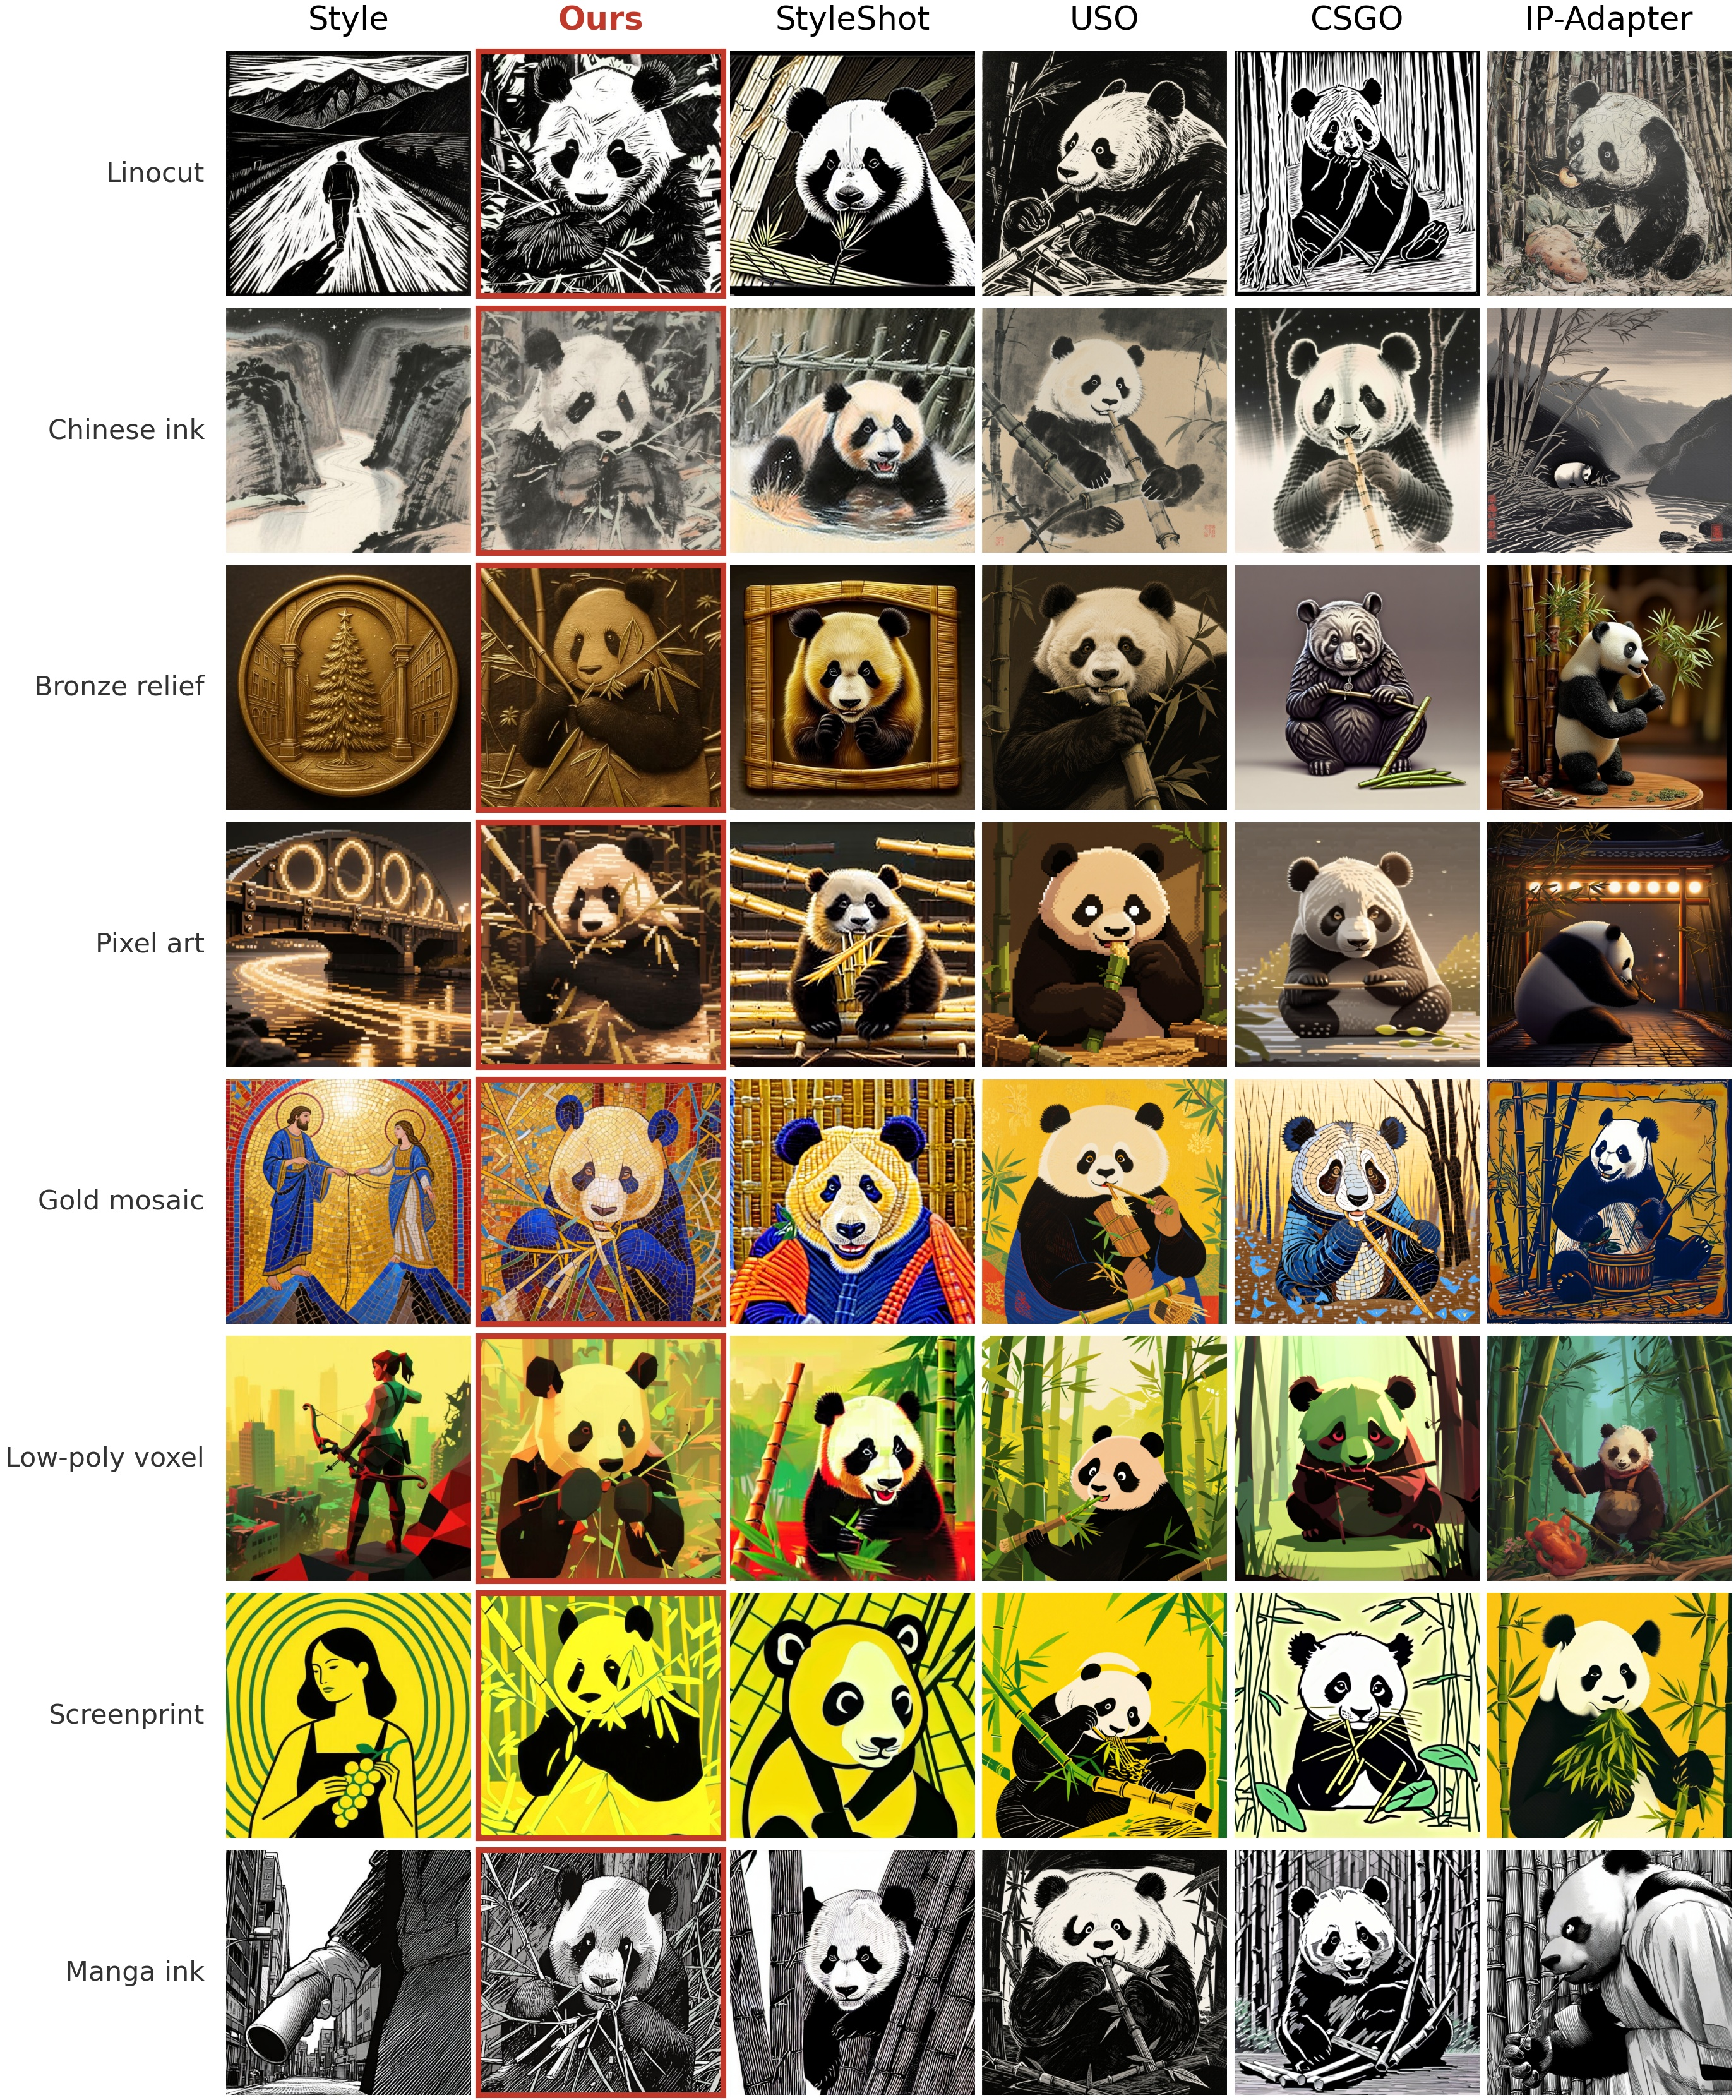
\includegraphics[width=.98\linewidth]{fig/figure/fig15_diverse_main.jpg}
  \caption{Qualitative comparison with four trained adapters across
    eight maximally distinct style families (prompt: ``A panda eat bamboo'');
    columns: style reference, Ours (Hyperion), StyleShot, USO, CSGO,
    IP-Adapter. Best viewed zoomed.}
  \label{fig:diverse_main}
\end{figure*}

\begin{table}[t]
  \centering
  % 十修: dropped stale "(prompt ``A panda eat bamboo'')" — that is the prompt of
  % the qualitative fig:diverse_main only; this table is a multi-prompt mean
  % (Ours: 6 prompts, baselines: 5), as now disclosed at the caption end.
  % 十修: Ours column recomputed as a 5-prompt mean (p0-p4, dropping p5) to match
  % the baselines' prompt set, from results/t2i_full_benchmark.csv
  % (method=hybrid2). Zero win/loss flips vs. the prior 6-prompt values
  % (still 19/21); shading P recomputed per-cell with the same formula below;
  % Mean 0.655 -> 0.657.
  \caption{Per-style-family CSD ($\uparrow$) across 21 diverse style media
  (mean over content prompts). Best per row in
  \textbf{bold}; cell shading encodes the CSD value on a single scale
  across the whole table (darker = higher). Our training-free Hyperion leads on
  19/21 families; the two
  exceptions (manga, anime) go to IP-Adapter, which is tuned for character imagery.
  Ours is recomputed from the full seed-43 benchmark over the 5 prompts
  shared with the baselines (p0--p4); trained baselines are run at their
  native resolution (Sec.~\ref{app:trained_baselines}).}
  \label{tab:percat}
  \footnotesize
  \setlength{\tabcolsep}{4.5pt}
  \begin{tabular}{l ccccc}
  \toprule
  Style family & Ours & StyleShot & USO & CSGO & IP-Ad. \\
  \midrule
  % cell shading: P = (v-0.154)/(0.779-0.154)*55, one scale for the whole table
  Pop halftone     & \cellcolor{tabshade!43}\textbf{0.644} & \cellcolor{tabshade!37}0.580 & \cellcolor{tabshade!24}0.432 & \cellcolor{tabshade!18}0.363 & \cellcolor{tabshade!3}0.190 \\
  Screenprint      & \cellcolor{tabshade!47}\textbf{0.686} & \cellcolor{tabshade!41}0.616 & \cellcolor{tabshade!40}0.603 & \cellcolor{tabshade!27}0.463 & \cellcolor{tabshade!34}0.536 \\
  Ink storybook    & \cellcolor{tabshade!33}\textbf{0.530} & \cellcolor{tabshade!17}0.346 & \cellcolor{tabshade!17}0.349 & \cellcolor{tabshade!28}0.473 & \cellcolor{tabshade!32}0.515 \\
  Bronze relief    & \cellcolor{tabshade!38}\textbf{0.588} & \cellcolor{tabshade!23}0.421 & \cellcolor{tabshade!0}0.154 & \cellcolor{tabshade!5}0.206 & \cellcolor{tabshade!15}0.322 \\
  Impasto collage  & \cellcolor{tabshade!47}\textbf{0.683} & \cellcolor{tabshade!27}0.464 & \cellcolor{tabshade!36}0.565 & \cellcolor{tabshade!34}0.544 & \cellcolor{tabshade!10}0.266 \\
  Embroidery       & \cellcolor{tabshade!49}\textbf{0.709} & \cellcolor{tabshade!33}0.526 & \cellcolor{tabshade!28}0.472 & \cellcolor{tabshade!45}0.668 & \cellcolor{tabshade!15}0.321 \\
  Linocut          & \cellcolor{tabshade!46}\textbf{0.672} & \cellcolor{tabshade!29}0.489 & \cellcolor{tabshade!36}0.559 & \cellcolor{tabshade!39}0.597 & \cellcolor{tabshade!9}0.259 \\
  Manga ink        & \cellcolor{tabshade!40}0.611 & \cellcolor{tabshade!24}0.428 & \cellcolor{tabshade!18}0.364 & \cellcolor{tabshade!35}0.550 & \cellcolor{tabshade!41}\textbf{0.622} \\
  Gold mosaic      & \cellcolor{tabshade!36}\textbf{0.558} & \cellcolor{tabshade!24}0.430 & \cellcolor{tabshade!10}0.267 & \cellcolor{tabshade!28}0.470 & \cellcolor{tabshade!8}0.246 \\
  Oil impasto      & \cellcolor{tabshade!49}\textbf{0.713} & \cellcolor{tabshade!35}0.553 & \cellcolor{tabshade!35}0.547 & \cellcolor{tabshade!43}0.639 & \cellcolor{tabshade!8}0.243 \\
  Blue screenprint & \cellcolor{tabshade!53}\textbf{0.751} & \cellcolor{tabshade!28}0.467 & \cellcolor{tabshade!33}0.527 & \cellcolor{tabshade!34}0.546 & \cellcolor{tabshade!34}0.539 \\
  Pixel art        & \cellcolor{tabshade!44}\textbf{0.656} & \cellcolor{tabshade!12}0.289 & \cellcolor{tabshade!23}0.411 & \cellcolor{tabshade!32}0.512 & \cellcolor{tabshade!26}0.448 \\
  Propaganda       & \cellcolor{tabshade!43}\textbf{0.645} & \cellcolor{tabshade!35}0.550 & \cellcolor{tabshade!26}0.455 & \cellcolor{tabshade!24}0.432 & \cellcolor{tabshade!6}0.220 \\
  Low-poly voxel   & \cellcolor{tabshade!51}\textbf{0.730} & \cellcolor{tabshade!42}0.633 & \cellcolor{tabshade!28}0.476 & \cellcolor{tabshade!46}0.672 & \cellcolor{tabshade!21}0.392 \\
  \midrule \multicolumn{6}{l}{\textit{Extended iconic families}}\\
  Anime cel        & \cellcolor{tabshade!44}0.654 & \cellcolor{tabshade!27}0.464 & \cellcolor{tabshade!25}0.442 & \cellcolor{tabshade!26}0.455 & \cellcolor{tabshade!48}\textbf{0.703} \\
  Chinese ink      & \cellcolor{tabshade!41}\textbf{0.618} & \cellcolor{tabshade!11}0.281 & \cellcolor{tabshade!29}0.489 & \cellcolor{tabshade!27}0.466 & \cellcolor{tabshade!32}0.516 \\
  Cyberpunk neon   & \cellcolor{tabshade!55}\textbf{0.782} & \cellcolor{tabshade!42}0.636 & \cellcolor{tabshade!37}0.575 & \cellcolor{tabshade!41}0.615 & \cellcolor{tabshade!41}0.616 \\
  Graffiti         & \cellcolor{tabshade!46}\textbf{0.678} & \cellcolor{tabshade!38}0.591 & \cellcolor{tabshade!14}0.318 & \cellcolor{tabshade!26}0.455 & \cellcolor{tabshade!19}0.366 \\
  Stained glass    & \cellcolor{tabshade!43}\textbf{0.638} & \cellcolor{tabshade!34}0.542 & \cellcolor{tabshade!31}0.503 & \cellcolor{tabshade!32}0.518 & \cellcolor{tabshade!30}0.492 \\
  Steampunk        & \cellcolor{tabshade!43}\textbf{0.640} & \cellcolor{tabshade!35}0.556 & \cellcolor{tabshade!31}0.504 & \cellcolor{tabshade!27}0.461 & \cellcolor{tabshade!30}0.499 \\
  Ukiyo-e          & \cellcolor{tabshade!41}\textbf{0.616} & \cellcolor{tabshade!23}0.416 & \cellcolor{tabshade!32}0.522 & \cellcolor{tabshade!33}0.527 & \cellcolor{tabshade!30}0.500 \\
  \midrule
  \textbf{Mean}    & \cellcolor{tabshade!44}\textbf{0.657} & \cellcolor{tabshade!29}0.489 & \cellcolor{tabshade!26}0.454 & \cellcolor{tabshade!31}0.506 & \cellcolor{tabshade!23}0.420 \\
  \midrule
  STM (mean)       & \textbf{0.738} & 0.695 & 0.405 & 0.567 & 0.569 \\
  \bottomrule
  \end{tabular}
\end{table}
% ─────────────────────────────────────────────────────────────────────────────

% ─────────────────────────────────────────────────────────────────────────────
\subsection{Output-Space Texture Coherence}
\label{sec:exp:texcoh}

CSD and the per-family results above measure style similarity in an embedding
space; we now verify that this advantage corresponds to a real, measurable
texture signature in the pixels rather than an artifact of one descriptor.
The spatial-neighbor cosine $\rho$ (Sec.~\ref{sec:method:gap}) showed that
backpropagation couples neighbouring \emph{latent updates} ($\rho{=}0.64$) where
per-token transport does not ($\rho{=}0.24$); we ask whether this coupling
survives into the \emph{output image}. For each output we compute two
parameter-free statistics: \textbf{texture energy}, the mean magnitude of the
high-pass residual $g-\mathrm{blur}(g)$, and \textbf{orientation coherence}, the
energy-weighted structure-tensor coherence
$(\lambda_1{-}\lambda_2)/(\lambda_1{+}\lambda_2)$ over $16\times16$ patches---how
strongly oriented (brushstroke-like) the local texture is.

Both statistics peak for our method and rank the pipeline variants in the same
order as CSD (Table~\ref{tab:texcoh}), correlating with CSD across the five
variants at Pearson $r{=}{+}0.97$ (energy) and $r{=}{+}0.88$ (coherence). The
update-space coupling that $\rho$ diagnoses therefore leaves a concrete
imprint---more energetic, more coherently oriented texture---making texture
coherence an \emph{output-space analogue of $\rho$} and independent corroboration
that our CSD gain reflects genuine brushstroke structure, not descriptor-specific
optimization. Like CSD, these measure texture \emph{presence}, not quality (a
method that over-textures would also score high), and must be read together with
the content metrics; we report LPIPS and ArtFID, and give the full analysis, in
Appendix~\ref{app:newmetrics}.

\paragraph{Style--Texture Match: a cross-method style metric}
Texture energy and orientation coherence validate our \emph{mechanism}, but they
measure texture \emph{presence}, so they cannot separate methods that produce
generic texture (a trained adapter textures too). We therefore introduce the
\textbf{Style--Texture Match (STM)}: the \emph{correlation} between the
orientation histogram of an output's high-pass residual and that of its
\emph{style reference}---a cosine taken after mean-centering both histograms, so
it measures the match of the texture-orientation \emph{profile} rather than the
dominant axis that all images share, averaged over pairs. STM
tracks CSD across our pipeline variants (Pearson $r{=}{+}0.98$) and, unlike raw
orientation coherence, \emph{also} discriminates sharply across \emph{trained}
methods: our training-free Hyperion attains the highest STM on both T2I
(Table~\ref{tab:percat}: $0.738$ vs.\ $0.41$--$0.70$) and I2I
(Table~\ref{tab:i2i_ext}: $0.716$ vs.\ $0.26$--$0.47$), confirming that it
reproduces the reference's specific texture orientations far more faithfully than
any baseline---trained or not. (The I2I table additionally reports the
style--content harmonic SCH, defined below, on which Hyperion also leads.)

\begin{table}[t]
  \centering
  \caption{Output-space texture analysis on the 40-sample T2I subset. Texture
           energy and orientation coherence (both $\uparrow$) peak for our method
           and track CSD across the five variants at $r{=}{+}0.97$ and
           $r{=}{+}0.88$. \textbf{Bold} $=$ best.}
  \label{tab:texcoh}
  \footnotesize
  \begin{tabular}{lccc}
    \toprule
    Method & Tex.\ energy~$\uparrow$ & Orient.\ coh.~$\uparrow$ & CSD \\
    \midrule
    \rowcolor{tabshade!10}
    \textbf{Ours (Hyperion)} & $\mathbf{0.075}$ & $\mathbf{0.622}$ & $0.681$ \\
    Adam-8                 & $0.074$ & $0.574$ & $0.650$ \\
    SLT-only               & $0.068$ & $0.587$ & $0.298$ \\
    Inject                 & $0.056$ & $0.492$ & $0.039$ \\
    Text-only              & $0.058$ & $0.503$ & $-0.011$ \\
    \bottomrule
  \end{tabular}
\end{table}

% ─────────────────────────────────────────────────────────────────────────────
\subsection{Image-to-Image Style Transfer}
\label{sec:exp:i2i}

We evaluate the I2I extension (Sec.~\ref{sec:method:i2i}) on the 40-pair
subset described in Sec.~\ref{sec:exp:setup} (8 styles $\times$ 5 content
images), reporting CSD, CLIP-T, CLIP-I, STM, and forward passes per step; the
per-method ablation table is in the supplement (Table~\ref{tab:i2i}).

The I2I Hyperion configuration (\texttt{ADAIN\_ALPHA}$=0.3$,
\texttt{START\_TIME}$=870$) achieves CSD~$=0.696$ with 4 forward passes,
substantially higher than both the AdaIN floor ($0.155$) and Adam-8 ($0.649$, 10 fwd),
while maintaining competitive CLIP-I~$=0.670$ (vs.\ $0.695$ for Adam-8),
confirming that the SLT pre-alignment step transfers cleanly to
image-conditioned inputs.
The CSD--CLIP-I Pareto scatter (Fig.~\ref{fig:i2i_scatter} in the
supplementary) confirms that Hyperion occupies the top-left region, achieving
the best style--content trade-off among all methods.

On the full 741-pair I2I benchmark, Hyperion attains CSD~$= 0.662$ and
CLIP-I~$= 0.650$, consistent with the 40-pair subset above.
We further compare against Klein's \emph{native} in-context image edit
(prompting the backbone to restyle the content directly): it reaches only
CSD~$= 0.487$ and is unreliable, failing (CSD~$< 0.30$) on $25\%$ of pairs
versus $0\%$ for Hyperion, motivating an explicit style-transfer pipeline over
the backbone's built-in editing (qualitative examples in the supplement,
Fig.~\ref{fig:native_cmp}).

Qualitative examples (supplement, Fig.~\ref{fig:i2i_qual}) show that content
structure (identity, pose, layout) is well preserved while brushstroke
texture and color palette are faithfully transferred.

\paragraph{Comparison with trained style-transfer methods}
We benchmark Hyperion against four \emph{trained} baselines in the same
content$+$style I2I setting: the SDXL adapters CSGO~\cite{xing2024csgo} and
IP-Adapter~\cite{ipadapter2023}, the FLUX adapter USO~\cite{wu2025uso}, and the
instruction-edit model Qwen-Image-Edit, evaluated with CSD, CLIP-I, LPIPS,
FID, and ArtFID~\cite{wright2022artfid} (Table~\ref{tab:i2i_ext}; qualitative
comparison in the supplement, Fig.~\ref{fig:i2i_ext}); our entries are averaged
over four seeds. Because these methods trade style fidelity against content
preservation, we summarize the balance with the \emph{Style--Content Harmonic}
$\mathrm{SCH}=\sqrt{\mathrm{CSD}\cdot\mathrm{CLIP\text{-}I}}$, which rewards
methods that transfer style \emph{and} preserve content while penalizing
degenerate behaviour at either extreme.
Our training-free Hyperion attains the \emph{highest} style fidelity
(CSD~$=0.712$) of all methods---above the trained adapters CSGO ($0.557$) and
USO ($0.510$), and far above IP-Adapter ($0.160$), whose image-prompt adapter
applies only a generic painterly cast that barely matches the specific
reference---and the highest SCH ($0.686$).
Measured with a small-sample-appropriate Inception feature (the default
$2048$-d FID is rank-deficient at $n{=}40$), our Hyperion also attains the best
distributional scores---FID $5.4$ and ArtFID $10.9$, ahead of Qwen-Image-Edit
($7.5$/$14.1$) and the adapters---so it leads on \emph{every} axis except raw
content preservation, where redrawing less of the image (IP-Adapter, USO) trades
away style. A training-free pipeline on a frozen backbone thus reaches the best
style--content balance of any method tested, trained or not.

\begin{table*}[t]
  \centering
  \caption{I2I comparison with \emph{trained} style-transfer methods (40-pair
    subset; our entries averaged over 4 seeds). SCH is the style--content
    harmonic (defined above); STM is the Style--Texture
    Match (Sec.~\ref{sec:exp:texcoh}). Our training-free Hyperion leads on style
    fidelity (CSD), on the balanced SCH, on STM, and on FID/ArtFID. FID/ArtFID
    use the $64$-d Inception feature, appropriate for the $40$-pair sample
    (the default $2048$-d estimate is rank-deficient and inflated at this $n$).
    \textbf{Bold} $=$ best.}
  \label{tab:i2i_ext}
  \footnotesize
  \begin{tabular}{lccccccc}
    \toprule
    Method & CSD$\uparrow$ & CLIP-I$\uparrow$ & LPIPS$\downarrow$ & FID$\downarrow$ & ArtFID$\downarrow$ & SCH$\uparrow$ & STM$\uparrow$ \\
    \midrule
    CSGO (SDXL)        & 0.557 & 0.689 & 0.656 & 15.1 & 26.7 & 0.619 & 0.363 \\
    USO (FLUX)         & 0.510 & \textbf{0.766} & 0.666 & 8.9 & 16.5 & 0.625 & 0.263 \\
    IP-Adapter (FLUX)  & 0.160 & 0.623 & \textbf{0.558} & 17.0 & 28.0 & 0.316 & 0.465 \\
    Qwen-Image-Edit    & 0.343 & 0.708 & 0.663 & 7.5 & 14.1 & 0.493 & 0.405 \\
    \rowcolor{tabshade!10}
    \textbf{Ours (Hyperion)} & \textbf{0.712} & 0.660 & 0.696 & \textbf{5.4} & \textbf{10.9} & \textbf{0.686} & \textbf{0.716} \\
    \bottomrule
  \end{tabular}
\end{table*}


% ─────────────────────────────────────────────────────────────────────────────
\subsection{Efficiency Analysis}
\label{sec:exp:efficiency}

% 十一修 评阅#6: 以下 "Iteration-count trade-off" 段与 tab:iter_tradeoff 表自
% Sec.3.4（Adam-in-Loop）整体移入本小节；内文仅新写首句衔接（\REV），其余文字
% 与十修版一致（含 B11 选择规则的 \REV 块）。
\paragraph{Iteration-count trade-off}
We first quantify the effect of the Adam iteration count $N$ inside each
active denoising step (Sec.~\ref{sec:method:adam}).
Table~\ref{tab:iter_tradeoff} shows that Hyperion exceeds Adam-only at every
iteration count and equal forward-pass budget; both improve monotonically with
diminishing returns beyond $N=5$ (at $N=8$ Hyperion reaches CSD~$= 0.766$ vs.\
Adam-only's $0.738$ on this aggressive-config 40-sample subset), with genuine
brushstroke texture visible in qualitative outputs.
The Adam-8 reference baseline reported in Tables~\ref{tab:main}
and~\ref{tab:ablation} uses a more conservative configuration
(lr$\,{=}\,0.01$, $w_c{=}0.2$), reaching CSD~$= 0.608$ on the full benchmark
and $0.650$ on the ablation subset---in both cases far above best-effort
injection.
% 十修: B11 — selection rule for the conservative Adam-8 baseline, derived from
% results/t2i_adam_only_sweep.csv (aggressive N=8: CSD 0.738 but CLIP-T 0.231).
The conservative configuration is chosen as the reference because it is
the strongest Adam-only setting that still operates at content preservation
comparable to ours (CLIP-T $0.296$--$0.299$ vs.\ our $0.294$--$0.296$); the
aggressive sweep configuration at $N{=}8$ buys its higher CSD ($0.738$) at
CLIP-T~$=0.231$, a content degradation far outside the operating range, and
would make the efficiency comparison style-for-content rather than
like-for-like.
However, wall time grows proportionally (each Adam iteration requires one full
model forward pass and one backward pass), reaching $\approx 19$~s at $N=8$.
CLIP-T degrades with more iterations as style pressure accumulates
against content structure.

\begin{table}[h]
  \centering
  \caption{Iteration cost vs.\ quality on the sweep configuration (40-sample
           subset, 8 styles $\times$ 5 prompts, seed~43; aggressive sweep
           hyperparameters lr$\,{=}\,0.03$, $w_s{=}2.0$, $w_c{=}1.5$).
           Hyperion (SLT pre-alignment $+$ Adam) exceeds Adam-only at
           \emph{every} iteration count and equal forward-pass budget, with the
           largest margin at the $N{=}2$ operating point.
           Absolute levels here run above the conservative main-table
           configuration (Table~\ref{tab:main}); the per-$N$ ranking, not the
           level, is the point.}
  \label{tab:iter_tradeoff}
  \footnotesize
  \begin{tabular}{lccc}
    \toprule
    $N$ & Hyperion CSD~$\uparrow$ & Adam-only CSD~$\uparrow$ & Fwd./step~$\downarrow$ \\
    \midrule
    2   & \textbf{0.682} & 0.582 & 4  \\
    5   & \textbf{0.744} & 0.700 & 7  \\
    8   & \textbf{0.766} & 0.738 & 10 \\
    \bottomrule
  \end{tabular}
\end{table}

% 十一修 评阅#6 追加: 原 Sec.3.8 的 Results 段并入于此（去重后浓缩：全基准
% +5.2% 已在 Sec.4.2，N≈4 追平论述已在下方 operating-point 句）。
\paragraph{Equal-budget comparison}
On the 40-sample ablation subset, Hyperion reaches CSD~$= 0.681$,
CLIP-T~$= 0.274$ with 4 forward passes per denoising step ($\approx 6.4$~s):
\textbf{+4.8\%} CSD over Adam-8 on the same subset ($0.650$, 10 forward
passes) at $2.5\times$ lower forward-pass cost.
At equal compute budget (same 4 forward passes), Hyperion outperforms
Adam-only by \textbf{+16.6\%} CSD ($0.681$ vs.\ $0.584$), confirming that SLT
pre-alignment, not iteration count, is the key enabler.

\paragraph{Wall-clock timing}
Wall-clock timing on a single H200 GPU corroborates the forward-pass advantage.
SLT alone adds negligible overhead (2.2~s $\approx$~baseline); the Hyperion
pipeline at $N=2$ Adam iterations runs in 6.4~s, achieving a $3.0\times$
speedup over Adam$\times$8 (19.0~s) while exceeding its style fidelity
(CSD~$=0.640$ vs.\ $0.608$, Table~\ref{tab:main}); a per-method timing
breakdown appears in the supplement (Fig.~\ref{fig:timing}).
Fig.~\ref{fig:iter_tradeoff} plots the full CSD vs.\ wall-clock trade-off:
the Hyperion front dominates the Adam-only front at every compute budget.
The operating point (two Adam iterations, $6.4$~s) reaches CSD~$0.682$ on
this subset, a level Adam-only first attains at $\approx 10.6$~s
($N{=}4$)---a $\sim 2\times$ iteration-efficiency gain from SLT
pre-alignment; SLT-only is the zero-iteration lower bound. Absolute CSD on
the subset runs above the conservative full-benchmark numbers of
Table~\ref{tab:main}; the Pareto shape, not the level, is the point.

\begin{figure}[H]
  \centering
  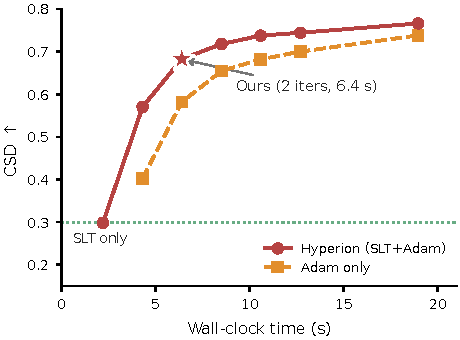
\includegraphics[width=\linewidth]{fig/figure/fig2_pareto.pdf}
  \caption{CSD vs.\ wall-clock trade-off (40-sample subset): Hyperion
    (red) vs.\ Adam-only (orange); $\star$ marks the operating point.}
  \label{fig:iter_tradeoff}
\end{figure}

% ─────────────────────────────────────────────────────────────────────────────
\subsection{Cross-Backbone Generalization}
\label{sec:exp:backbone}

Our Hyperion pipeline targets the MM-DiT family of architectures, which shares the same double-stream self-attention design across models.
To verify generalization, we apply the identical pipeline---same hyperparameters, no retuning---to FLUX.1-dev~\cite{flux2024} (12B parameters), a second MM-DiT model distinct from Klein~9B used in all other experiments.
On the same 40-sample subset (8 styles $\times$ 5 prompts), FLUX.1-dev achieves CSD~$= 0.719$ and CLIP-T~$= 0.291$, versus Klein's CSD~$= 0.681$ and CLIP-T~$= 0.274$.
The higher scores on FLUX.1-dev are consistent with its larger capacity; the key finding is that the pipeline requires no modification.
Full details are in Appendix~\ref{app:flux1dev}.

A T2I benchmark gallery of Hyperion results across diverse styles and content
prompts is provided in the supplement (Fig.~\ref{fig:t2i_benchmark}).
